\chapter{Аналитический раздел}

В данном разделе рассмотрены основные термины предметной области восстановления дефокусированных изображений. Приведен обзор методов восстановления с учетом априорной информации об искажении, а также сравнительный анализ методов <<слепой>> деконволюции. Приведены методы оценки качества восстановления дефокусированных цифровых изображений.

\section{Терминология предметной области}

\subsection{Фотоаппарат}

Фотоаппарат --- это прибор для получения на фотографическом материале действительного изображения предмета при фотографировании~\cite{def1}.

Цифровой фотоаппарат --- фотоаппарат, в котором для регистрации изображения используется фотоэлектрический принцип.

Среди фотоаппаратов, выпускающихся в настоящее время, данный тип является значительно более распространенным (пленочными фотоаппаратами, в основе которых лежит химическая обработка фотоматериалов, пользуется менее 1\% населения)~\cite{dp_percent}, поэтому в данной работе будут рассматриваться изображения, полученные с помощью данного типа фотоаппаратов.

На рисунке \ref{camera} представлены основные элементы классического цифрового фотоаппарата.

\begin{figure}[H]
	\centering
	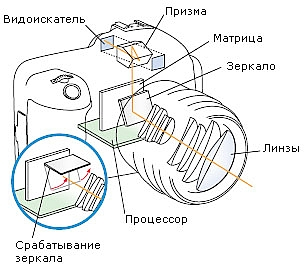
\includegraphics[scale=0.85]{assets/camera.jpg}
	\caption{Основные элементы цифрового фотоаппарата}
	\label{camera}
\end{figure}

Наиболее важным элементом с точки зрения рассмотрения вопроса дефокусировки является \textit{объектив} фотоаппарата, представляющий собой оптическую систему, состоящую из совокупности центрированных линз и диафрагмы, заключенных в общую оправу. Свет, проходящий через объектив, попадает на зеркало, после чего, отразившись в призме через видоискатель, попадает в глаз.

Основными характристиками объектива являются:

\begin{enumerate}
	\item Фокусное расстояние --- расстояние от оптического центра объектива до фокальной плоскости (матрицы), где происходит фокусировка света. Увеличение расстояния от предмета до линзы влечет за собой уменьшение расстояния от его изображения до линзы, и наоборот. Указанное условие обеспечивается фокусировкой объектива фотоаппарата перед съемкой~\cite{obj}.
	%Чем меньше фокусное расстояние, тем шире угол обзора и наоборот.
	\item Диафрагма --- система подвижных лепестков, формирующих отверстие определенного размера, регулирующее поток света, поступающий на светочувствительную матрицу, которая в свою очередь регистрирует этот поток и преобразует его в электрический сигнал. Данные, полученные с матрицы, после обработки записываются на карту памяти фотоаппарата.
\end{enumerate}

Каждый тип объектива имеет свои особенности и подходит для разных ситуаций съемки.

\subsection{Цифровое изображение}

Изображение, получаемое фотокамерой, можно определить как двумерную функцию $f(x,\;y)$, где $x$ и $y$ --- пространственные координаты. Значение функции $f$ в некоторой точке, задаваемой парой координат $(x, y)$, является положительной скалярной величиной, называемой интенсивностью, или яркостью (уровнем серого) изображения в этой точке~\cite{digital_pic}~\cite{digit_pic}.

Для изображений, получаемых цифровой фотокамерой, величины $x,\;y$ и $f$ принимают конечное число дискретных значений. Такие изображения называются цифровыми.

\clearpage

\subsection{Причины дефокусировки фотокамеры}

На рисунке \ref{schema} приведена схема~\cite{scheme}, иллюстрирующая физический принцип получения дефокусированного изображения.

\begin{figure}[H]
	\centering
	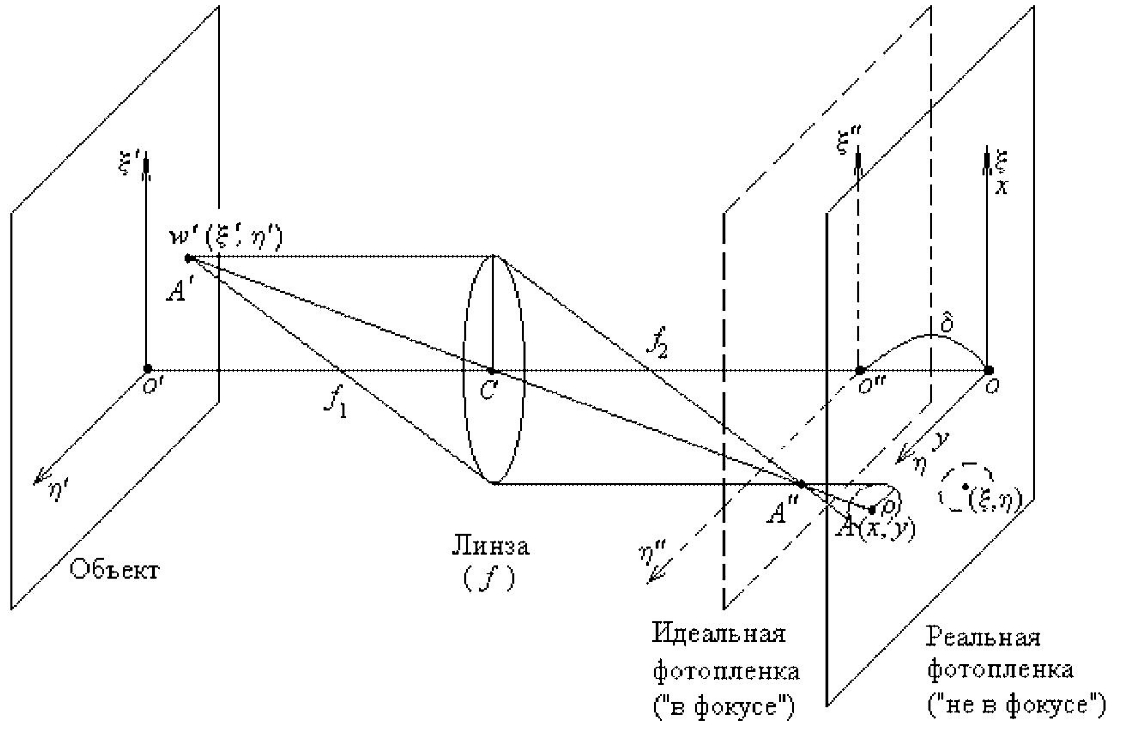
\includegraphics[scale=0.55]{assets/schema}
	\caption{Принцип получения дефокусированного изображения}
	\label{schema}
\end{figure}

Пусть снимаемый объект, полагаемый плоским из-за его удаленности, и фотопленка (или матрица сенсоров) расположены параллельно тонкой линзе по разные стороны от нее. Пусть $\delta$~---~погрешность фокусировки изображения, $f_1$~---~расстояние от линзы до объекта, $f_2$~---~расстояние от линзы до фотопленки (матрицы), установленной в <<фокусе>> ($\delta = 0$).

Как видно из рисунка, лучи из точки $A'$ после их прохождения через линзу отобразятся на реальной фотопленке не в точку, а в некоторое размытое пятно радиуса $\rho = \cfrac{a\delta}{f_2}$ с центром в точке $A(x,\;y)$, где $a$ --- радиус апертуры линзы. Данное пятно определяется т.~н. функцией рассеяния точки, или функцией искажения ядра.

Дефокусированным изображением называется изображение, полученное на реальной пленке (<<не в фокусе>>) при $\delta \neq 0$.

\clearpage

\subsection{Функция рассеяния точки}

Функция рассеяния точки (англ. Point Spread Function) описывает, как оптическая система формирует изображение при наблюдении точечного источника или точечного объекта.

На рисунке \ref{psf_img} представлен пример формирования изображения.

\begin{figure}[H]
	\centering
	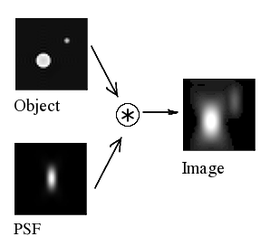
\includegraphics[scale=0.9]{assets/psf.png}
	\caption{Пример формирования изображения}
	\label{psf_img}
\end{figure}

Степень рассеяния является мерой качества системы формирования изображений. В зависимости от типа рассеивания ФРТ может быть приближена некоторыми распространенными математическими моделями, например гауссова функция или функция Эйри, также ФРТ может быть синтезирована на основе априорной информации о ее характере. Выбор конкретной модели функции рассеяния точки зависит от характеристик системы и требований к точности моделирования.

Опишем математически задачу дефокусировки. Рассмотрим помимо круга с центром $A(x,\;y)$ некоторый другой круг с центром в точке $(\xi,\;\eta)$. Радиусы этих (и других) кругов одинаковы и равны $\rho$, а их площади соответственно $\cfrac{\pi}{\rho^2}$. В результате некоторая интенсивность $w(\xi,\;\eta)$, соответствующая точке $(\xi,\;\eta)$, будет распределена по кругу радиуса $\rho$ и площади $S = \cfrac{\pi}{\rho^2}$ с плотностью интенсивности $\cfrac{w(\xi,\;\eta)}{\pi\rho^2}$, постоянной в пределах круга в первом приближении. 

Интенсивность в точке $A$ будет результатом суммирования (интегрирования) по всем тем кругам, которые накрывают точку $A(x,\;y)$. Условие накрытия точки кругом с центром в точке и радиуса $\rho$ имеет следующий вид:

\begin{equation}
	\sqrt{(x - \xi) ^ 2 + (y - \eta)^2} \leq \rho.
\end{equation}

В результате интенсивность в точке $A(x,\;y)$:

\begin{equation}
	g(x,\;y) = \iint_{\sqrt{(x - \xi) ^ 2 + (y - \eta)^2}^{} \leq \rho} \cfrac{w(\xi,\;\eta)}{\pi\rho^2} d\xi d\eta.
\end{equation} 

Соотношение (1.2) есть \textit{двумерное интегральное уравнение $I$ рода относительно $w(\xi,\;\eta)$}, однако оно записано в нестандартной форме. Приведем его к стандартной форме:

\begin{equation}
	\int_{-\infty}^{\infty}\int_{-\infty}^{\infty} k(x - \xi, \; y - \eta) w(\xi,\;\eta)d\xi d\eta = g(x,\; y), -\infty < x, y < \infty,
\end{equation}

где 

\begin{equation}
	k(x - \xi, \; y - \eta) = \begin{cases}
		\cfrac{1}{\pi\rho^2}\ , & \sqrt{(x - \xi) ^ 2 + (y - \eta)^2} \leq \rho,\\
		0, & \text{иначе}.
	\end{cases}
\end{equation}

Или 

\begin{equation}
	k(x, \; y) = \begin{cases}
		\cfrac{1}{\pi\rho^2}\ , & \sqrt{x ^ 2 + y^2} \leq \rho,\\
		0, & \text{иначе}.
	\end{cases}
\end{equation}

Соотношение (1.5) есть \textit{двумерное интегральное уравнение Фредгольма $I$ рода типа свертки}. Ядро интегрального уравнения $k(x,\;y)$ называется \textit{функцией рассеяния точки}.

Таким образом, установлено, что в случае дефокусировки ФРТ имеет вид диска~\cite{diskk} радиуса $\rho$ и интенсивностью внутри диска равной $\cfrac{1}{\pi\rho^2}$. Дальнейшая задача заключается в нахождении радиуса этого диска для последующего восстановления искажения.

\clearpage

%\subsection{Модели изображений}

%Модель цифрового изображения определяет как оно будет представлено и обработано в цифровой форме.
%
%\begin{enumerate}
%	\item Черно--белая модель Bitmap (Raster) --- модель, которая представляет изображение как набор пикселей, каждый из которых имеет свой цвет и расположен на определенной позиции на изображении.
%	\item Полутоновые изображения (grayscale) ---
%	\item Индексированный цвет ---
%	\item Полноцветные изображения ---
%\end{enumerate}

%\clearpage

\subsection{Основные цветовые модели}

Цифровая модель цифрового изображения --- это математическая модель, используемая для представления цвета на компьютере или ином цифровом устройстве. Она определяет способ представления цвета в цифровой форме.

\begin{enumerate}
	\item Модель \textit{RGB} (англ. Red, Green, Blue --- Красный, Зеленый, Синий) --- аддитивная цветовая модель, использующая три основных цвета для кодирования цифрового изображения. Выбор основных цветов обусловлен особенностями восприятия цвета человеческим глазом. 
	
	Данная модель используется для создания цветов на электронных устройствах: телевизоры, компьютеры, планшеты, смартфоны и т.д. 
	
	Цветовое пространство модели можно представить в виде куба, координатными осями которого являются красный, синий и зеленый цвета. Диагональ куба даст градации серого. На рисунке \ref{rgb_cube} представлен пример такого куба.
	
	\begin{figure}[H]
		\centering
		\includegraphics[scale=0.55]{assets/rgb_color_cube.pdf}
		\caption{Цветовое пространство RGB~--~модели}
		\label{rgb_cube}
	\end{figure}

	В современных системах каждая из этих компонент представлена в 255 градациях, что порождает около 16 млн различных оттенков. Однако, несмотря на размер цветового пространства, цветовой диапазон ограничен --- RGB не может воспроизвести многие воспринимаемые человеческим глазом цвета (например, спектрально чистый голубой), что может стать проблемой при работе с профессиональными цифровыми изображениями.
	
	Также недостатком данной модели является применимость только к линейным алгоритмам обработки. В противном случае данная модель не подходит.
	
	\clearpage
	
	\item Модель \textit{CMYK} (англ. Cyan, Magenta, Yellow, blacK --- Голубой, Пурпурный, Желтый, Черный) --- субтрактивная модель, используемая в типографии. 
	
	Основные цвета модели образовались при смешивании основных цветов RGB модели:
	
	\begin{itemize}
		\item красный и зеленый цвета порождают желтый;
		\item красный и синий цвета порождают пурпурный;
		\item зеленый и синий порождают голубой.
	\end{itemize}
	
	Также в модели используется черный цвет в качестве дополнительного к первым трем с целью улучшения контрастности, глубины теней и экономии красок, т.к. смешивание основных цветов даст грязно~--~серый, но не черный цвет. 
	
	Цветовое пространство модели также можно представить в виде куба, координатными осями которого являются голубой, пурпурный и желтый цвета. На рисунке \ref{cmyk_cube} представлен пример такого куба.
	
	\begin{figure}[H]
		\centering
		\includegraphics[scale=0.55]{assets/cmyk_color_cube.pdf}
		\caption{Цветовое пространство CMYK~--~модели}
		\label{cmyk_cube}
	\end{figure}

	\item Модель \textit{HSL} (англ. Hue, Saturation, Lightness --- Тон, Насыщенность, Светлота) --- модель, использующая для определения цвета три параметра: тон, насыщенность и светлоту. 
	
	Эта модель часто используется в области обработки изображений и визуализации данных. Идея заключается в том, что человеческий глаз в большей степени воспринимает изменение интенсивности и в меньшей --- изменение цвета, как в RGB.
	
	Цветовое пространство данной модели можно представить в виде двух симметричных конусов, расположенных на одной оси. На рисунке \ref{hsl_model} представлен пример таких конусов. На оси конусов отсчитывается интенсивность от черного до белого. По окружности отсчитывается тон. Вдоль радиуса откладывается насыщение.
	
	\begin{figure}[H]
		\centering
		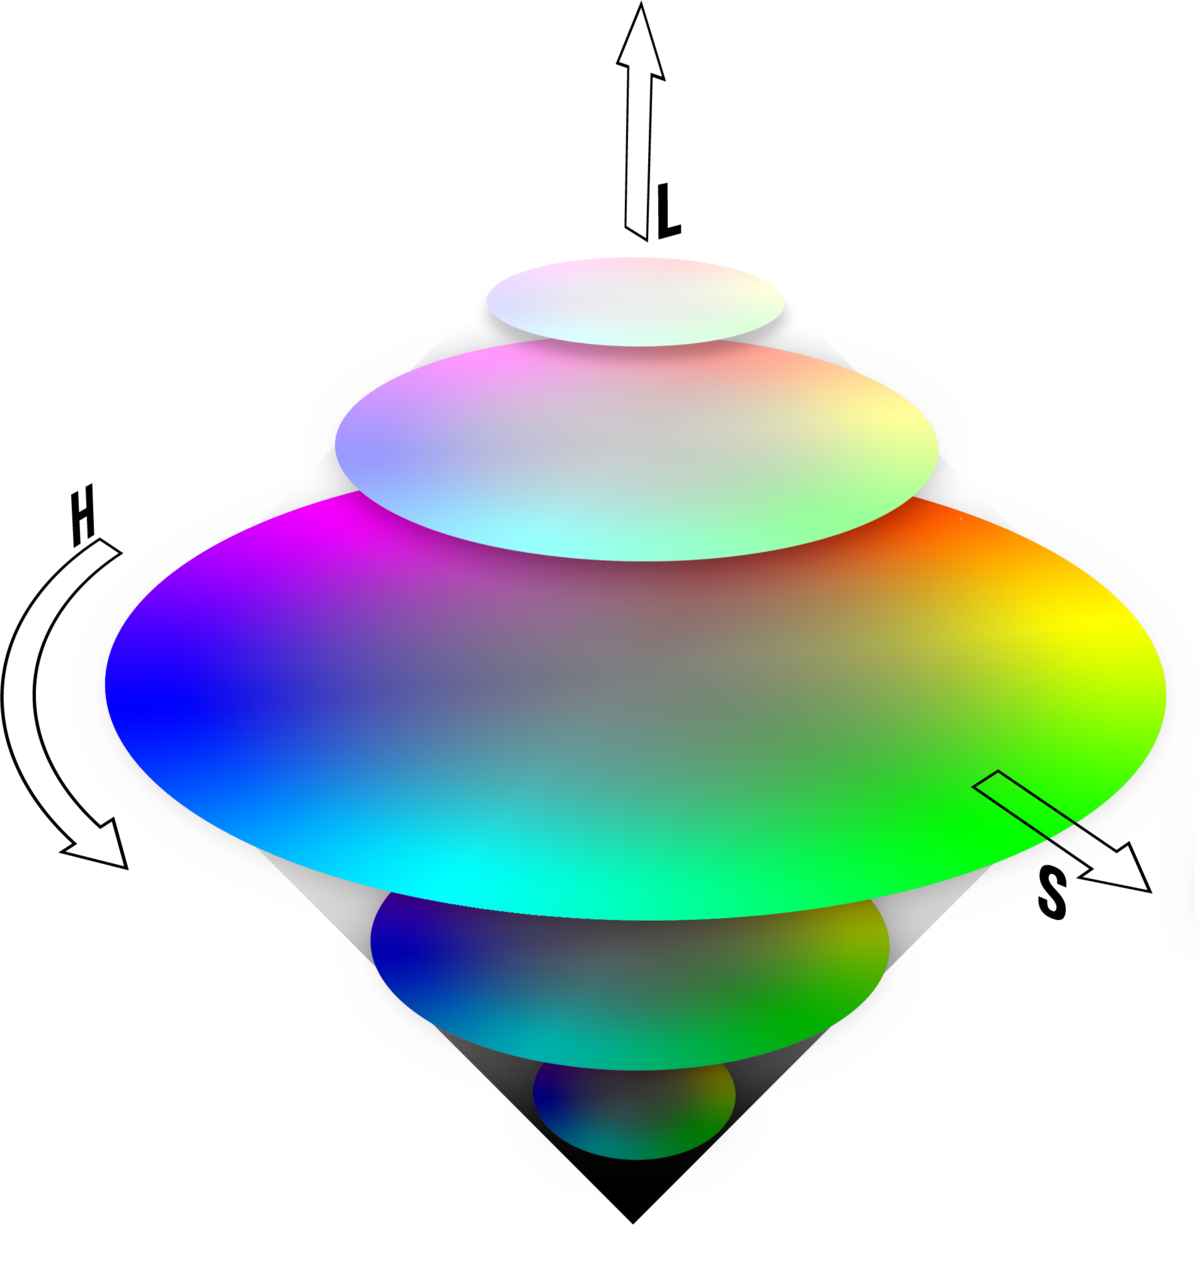
\includegraphics[scale=0.25]{assets/hsl_cone.png}
		\caption{Цветовое пространство HSL~--~модели}
		\label{hsl_model}
	\end{figure}
	
\end{enumerate}

\subsection{Основные форматы файлов изображения}

Формат файла изображения определяет способ хранения и передачи информации. Как известно, цифровое изображение, полученное с помощью фотоаппарата, не может быть векторным. Ниже приведены наиболее распространенные форматы файлов растрового изображения:

\begin{itemize}
        \item \textbf{BMP} (англ. Bitmap --- битовая карта) --- формат хранения однослойных растровых изображений. Данный способ записи не сжимает исходную информацию.
	\item \textbf{TIFF} (англ. Tagged Image File Format --- формат файла изображения с тегами) --- формат хранения высококачественных растровых изображений. Такие файлы могут содержать множество слоев, включая изображения, метаданные, цветовые профили и другую информацию, что делает их полезными для профессиональных приложений в графическом дизайне, фотографии и печати. 
	\item \textbf{JPEG} (англ. Joint Photographic Experts Group --- объединенная группа экспертов по фотографии) --- использует метод сжатия с потерями, однако размер таких файлов существенно меньше, поэтому данный формат может быть предпочтителен в случае терпимости к потерям.
	\item \textbf{PNG} (англ. Portable Network Graphics --- портативная сетевая графика) --- распространенный формат хранения и передачи растровых изображений, использующий использует алгоритм сжатия без потерь, что означает, что изображение сохраняется точно в том же качестве, что и оригинал, без потери деталей или цветовой точности. Также этот формат предоставляет возможности для работа с прозрачными изображениями и характеризуется малым размером файла в результате сжатия.
\end{itemize}

Каждый формат имеет свои преимущества и недостатки. Выбор формата зависит от конкретных потребностей и требований, предъявленных к поставленной задаче.

\clearpage

\subsection{Фурье~--~анализ}

Идея, лежащая в основе Фурье~--~анализа, заключается в том, что периодическая функция $f(t)$ непрерывной переменной $t$, имеющая период $\tau$, может быть представлена в виде взвешанной суммы косинусов и синусов. Данная сумма, известная как \textit{ряд Фурье}, имеет следующий вид:

\begin{equation}\label{ryad}
	f(t) = \sum_{n=-\infty}^{+\infty}c_n\cdot e^{in{\textstyle \frac{2\pi}{\tau}} t},
\end{equation}

где $i = \sqrt{-1}$, а коэффициенты $c_n$ равны:

\begin{equation}
	c(n) = \cfrac{1}{\tau}\cdot \int_{-\frac{\tau}{2}}^{\frac{\tau}{2}}f(t)\cdot e^{in{\textstyle \frac{2\pi}{\tau}}}dt, n = 0, \pm1, \pm2,...
\end{equation}

Тот факт, что выражение \ref{ryad} есть разложение на синусы и косинусы, следует из формулы Эйлера:

\begin{equation}
	e^{i\theta} = \cos\theta + i\cdot\sin\theta,
\end{equation}

где $e$ --- число Эйлера (2,71828...).

Преобразование Фурье --- операция, сопоставляющая одной функции вещественной переменной другую функцию вещественной переменной, которая описывает коэффициенты при разложении исходной функции на гармонические колебания (элементарные составляющие) с разными частотами.

Пусть $f(x)$ --- одномерная произвольная функция. Преобразование Фурье для этой функции определяется выражением (\ref{fourier}):

\begin{equation}\label{fourier}
	F(u) = \cfrac{1}{2\pi}\cdot \int_{-\infty}^{+\infty}f(x)\cdot e^{-ixu}dx,
\end{equation}

где $u$ --- частотная переменная, $F(v)$ --- Фурье~--~образ, который в общем случае является комплексным. 

Обратное преобразование Фурье имеет следующий вид:

\begin{equation}\label{inv_fourier}
	f(x) = \cfrac{1}{2\pi}\cdot \int_{-\infty}^{+\infty}F(u)\cdot e^{ixv}du.
\end{equation}

Выражения \ref{fourier} и \ref{inv_fourier} составляют т.н. Фурье-пару. 

На рисунке \ref{fig:example} представлена связь между временной (или пространственной) и частотной областью вычислений.

\begin{figure}[H]
	\centering
	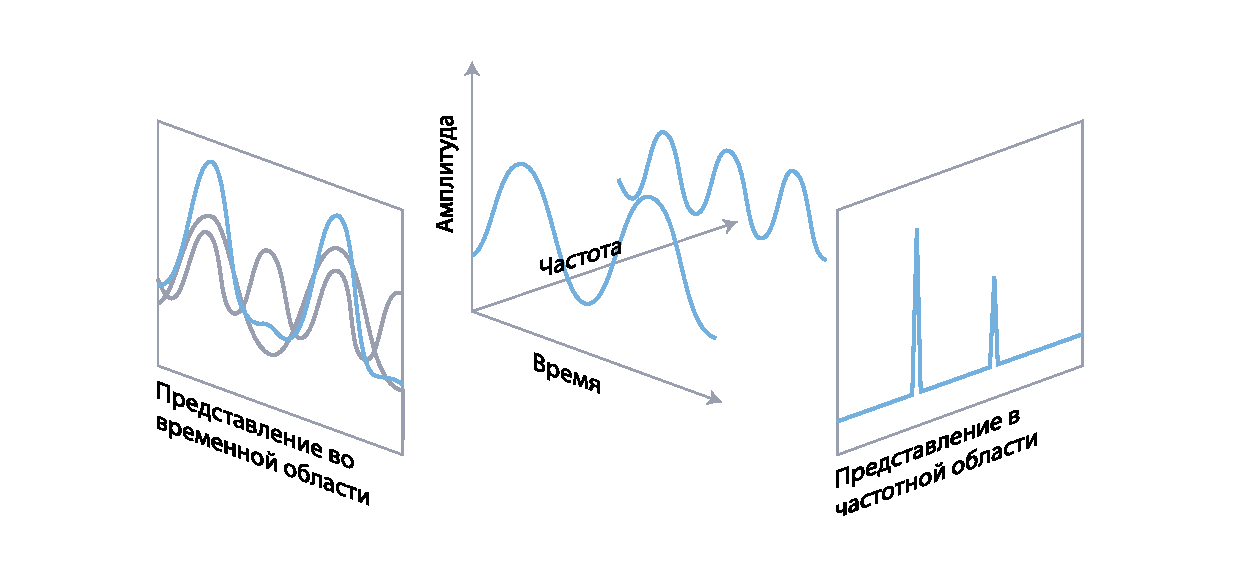
\includegraphics[scale=0.85]{assets/frequency-domain.pdf}
	\caption{Связь между временной и пространственной областью вычислений}
	\label{fig:example}
\end{figure}

Таким образом, для описания полного преобразования достаточно знать один полный период. Из этого следует, что обратным преобразованием Фурье можно восстановить $f(t)$ из единственного периода.

Эффективность применения рассматриваемого математического аппарата заключается в том, что функция, заданная преобразованием Фурье (или его рядом), \textit{может быть} полностью, восстановлена при помощи некоторой процедуры обращения. Таким образом, можно работать в т.н. Фурье~---~области, а затем вернуться в исходную область определения функции. 
%Также достоинством преобразования Фурье является тот факт, что оно может использоваться как для непрерывных функций, так и для дискретных.

Т.к. цифровая обработка сигналов основана на дискретизации и квантовании аналоговых сигналов, на практике необходимо обрабатывать конечное число отсчетов, вследствие чего было разработано аналогичное преобразование для дискретных сигналов --- дискретное преобразование Фурье, позволяющее восстановить непрерывный периодический сигнал. 

Прямое дискретное преобразование Фурье функции $f(x,\;y)$ цифрового изображения размерами $M\times N$ имеет следующий вид:

\begin{equation}\label{dpf}
	F(u,\;v)= \frac{1}{MN}\sum_{x=0}^{M-1}\sum_{y=0}^{N-1}f(x,\;y)\cdot e^{-2\pi i\textstyle(\frac{ux}{M}+\frac{vy}{N})},
\end{equation}

Обратное ДПФ изображения $f(x,\;y)$ имеет следующий вид:

\begin{equation}\label{dpf-inv}
	f(x,\;y) = \sum_{u=0}^{M-1}\sum_{v=0}^{N-1}F(u,\;v)\cdot e^{-2\pi i\textstyle(\frac{ux}{M}+\frac{vy}{N})}.
\end{equation}

Выражения \ref{dpf} и \ref{dpf-inv} составляют пару ДПФ.

Анализ сигналов, основанный на преобразовании сигнала из временной области в частотную область, называется \textit{спектральным}~\cite{spectrr}. Представление изображения в таком пространстве дает возможность наблюдать его структурные особенности, связанные с периодичностью повторения элементов, наличием мелких деталей и др.

На рисунках \ref{flowers} и \ref{flowers_full} представлены исходное изображение~\cite{flowers} и его спектр, являющийся результатом преобразования Фурье.

\begin{figure}[!htb]
	\begin{minipage}{0.5\textwidth}
		\centering
		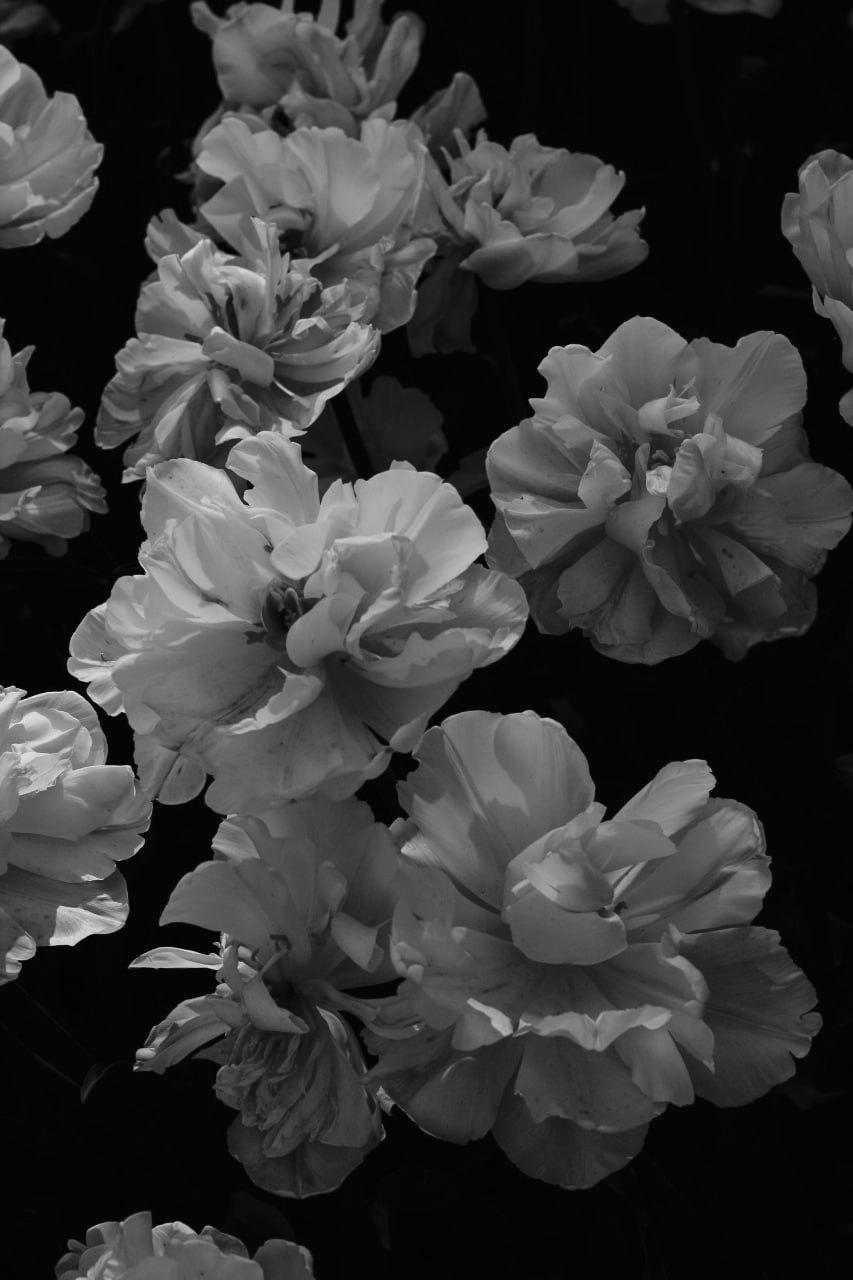
\includegraphics[scale=0.16]{assets/flowers_gray}
		\caption{Исходное изображение}\label{flowers}
	\end{minipage}\hfill
	\begin{minipage}{0.5\textwidth}
		\centering
		
\includegraphics[scale=0.22]{assets/flowers_gray_spectrum}
		\caption{Спектр изображения}\label{flowers_full}
	\end{minipage}
\end{figure}

Следует отметить, что в общем виде спектр сигнала является комплексным, однако в целях улучшения визуализации характерных особенностей сигнала рассматривают его амплитудный спектр, соответствующий реальной части комплексного числа, и фазовый, соответствующий мнимой части.

Выбор между анализом амплитудного или фазового спектра зависит от требований и ограничений в рамках решаемой задачи, однако в большинстве случаев амплитудный спектр является более распространенным инструментом анализа характеристик сигнала, т.к. он позволят определить, какие частоты присутствуют и какова их амплитуда, а также более прост в интерпретации.

\clearpage

На рисунках \ref{abs_flowers} и \ref{angle_flowers} представлены амплитудный и фазовый спектры исходного изображения. Здесь и далее спектры смещены в центр. В центре амлитудного спектра присутствует едва видимая белая точка.

\begin{figure}[!htb]
	\begin{minipage}{0.5\textwidth}
		\centering
		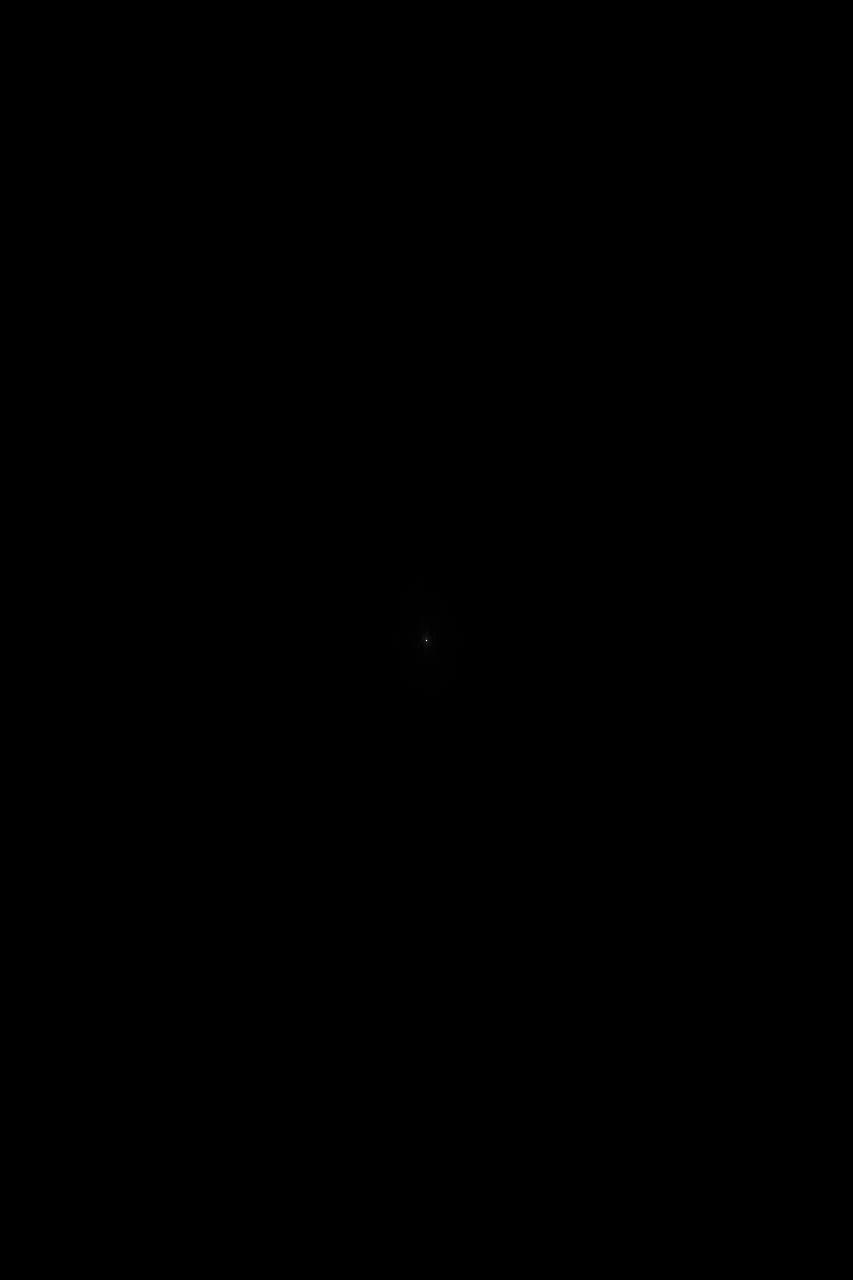
\includegraphics[scale=0.17]{assets/flowers_gray_abs_spectrum}
		\caption{Амплитудный спектр}\label{abs_flowers}
	\end{minipage}\hfill
	\begin{minipage}{0.5\textwidth}
		\centering
		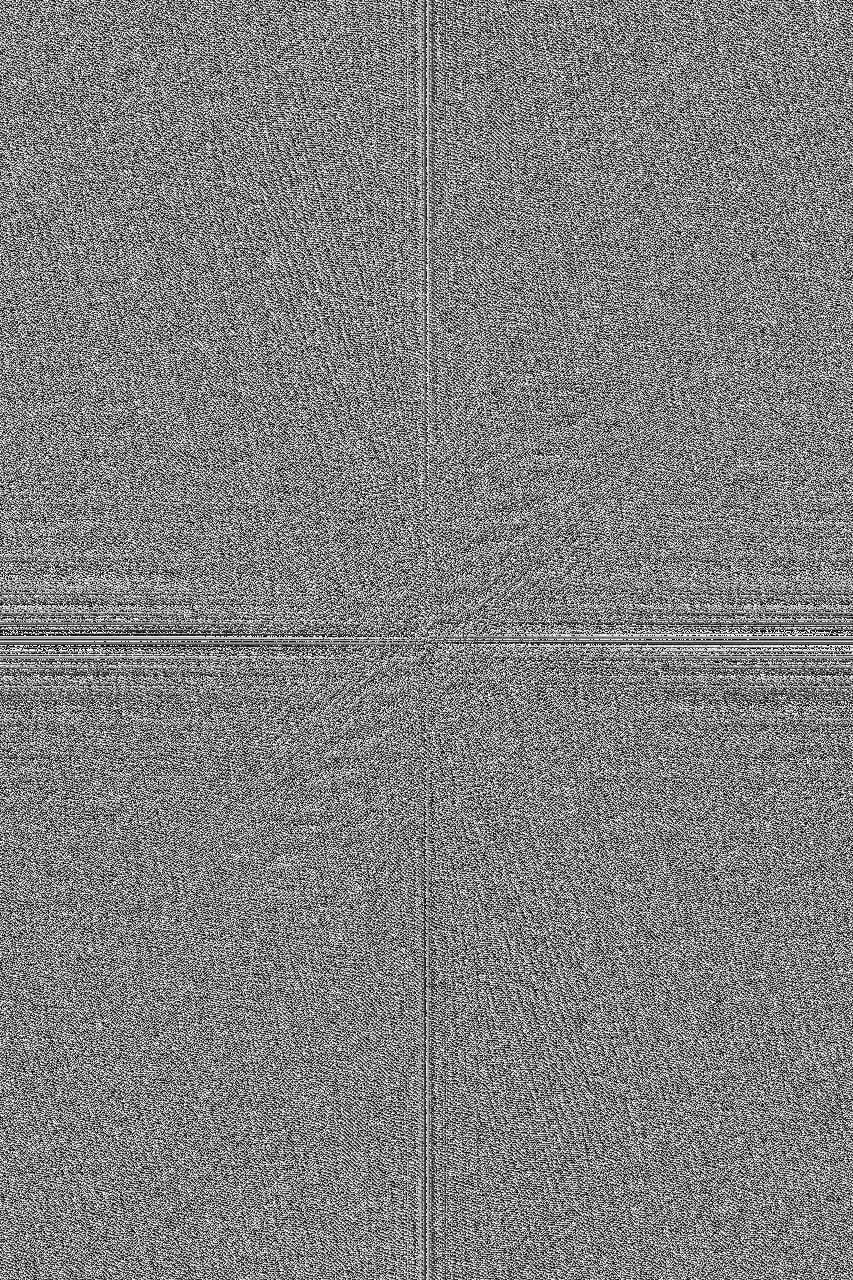
\includegraphics[scale=0.22]{assets/flowers_gray_angle_spectrum}
		\caption{Фазовый спектр}\label{angle_flowers}
	\end{minipage}
\end{figure}

Размерности амплитудного и фазового спектра всегда совпадают с размерностью исходного изображения.

Также существует \textit{кепстральный} анализ цифровых сигналов, основанный на применении преобразования Фурье к логарифму амплитудного спектра. 

Данный подход позволяет извлечь полезную информацию о спектральных характеристиках сигналов и обеспечивает новые возможности для анализа и обработки, которые не всегда могут быть доступны при использовании рассмотренного выше спектрального анализа. 

Кепстр~\cite{cepstrr}~\cite{ceps} изображения может быть представлен с помощью следующего выражения:

\begin{equation}
	C_s(u) = \ln|F(u)^2|,
\end{equation}

где $F(u)$ --- спектр сигнала.

\clearpage

На рисунке \ref{defocus_lena} представлено исходное дефокусированное изображение.

\begin{figure}[H]
	\centering
	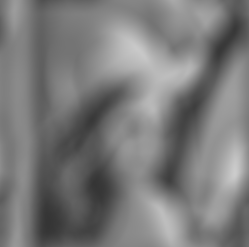
\includegraphics[scale=0.7]{assets/defocus}
	\caption{Дефокусированное изображение}
	\label{defocus_lena}
\end{figure}

На рисунках \ref{spect} и \ref{ceps} представлены амплитудные спектр и кепстр соответственно для искаженного изображения.

\begin{figure}[!htb]
	\begin{minipage}{0.5\textwidth}
		\centering
		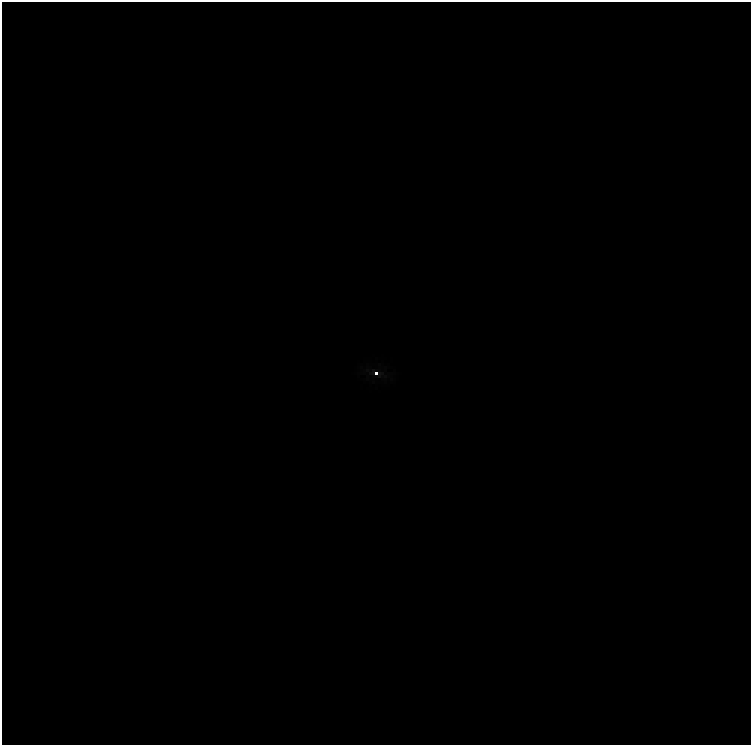
\includegraphics[scale=0.5]{assets/d2}
		\caption{Амплитудный спектр}\label{spect}
	\end{minipage}
	\begin{minipage}{0.5\textwidth}
		\centering
		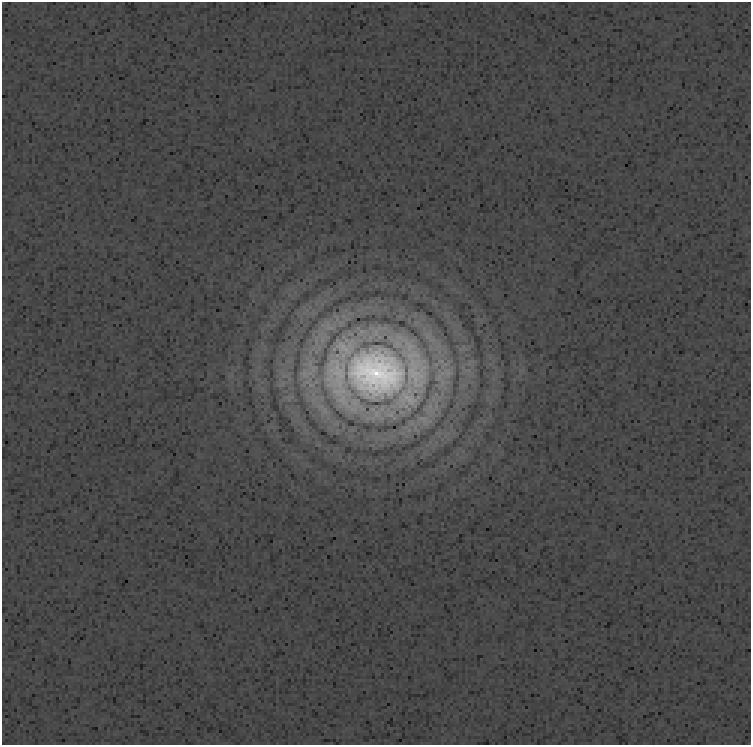
\includegraphics[scale=0.5]{assets/d1}
		\caption{Кепстр}\label{ceps}
	\end{minipage}
\end{figure}

Как можно заметить, если искажение сигнала вызвано дефокусировкой, то спектр сигнала также имеет яркую точку в центре, а кепстр будет содержать концентрические кольца~\cite{rings}.

\subsection{Шум}

Шум в цифровом сигнале представляет собой нежелательные случайные изменения полезного сигнала, которые могут вносить искажения и, следственно, ухудшать его качество. Эта помеха может существенно влиять на процесс обнаружения и извелечения значимой информации из сигнала, в частности, изображения.

Основными источниками шума на цифровом изображении являются сам процесс его получения (оцифровки), а также процесс передачи. Шум может быть как и аддитивным (не корреклирующим с изображением и не зависящим от координат пикселя), так и мультипликативным (изменяющим форму сигнала).

Выделяют следующие типы шума:

\begin{itemize}
	\item электронный шум, полученный вследствие теплового движения электронов в электронных частях снимающих систем;
	\item фотоэлектрический шум, возникающий в результате статистической природы света;
	\item шум, возникающий из-за зернистости фотопленки;
	\item дискретный шум, появляющийся при дискретизации изображения.
\end{itemize}

Для борьбы с шумом могут применяться различные методы фильтрации, такие как: медианный фильтр, фильтр среднего значения, фильтр Каламана и др. Одним из важных аспектов при обработке сигнала является достижение баланса между уровнем шума и сохранением полезной информации о сигнале.

\subsection{Свертка (конволюция)}

Применительно к обработке цифровых изображений операция свертки может быть интерпретирована следующим образом: на основе некоторого множества пикселей исходного изображения вычисляется новый пиксель результирующего (искаженного ядром свертки) изображения.

В зависимости от выбранного ядра свертки, применяемого к изображению, можно получить тот или иной эффект: размытость, повышение резкости, обнаружение контуров, граничное обнаружение и т.~д.

Математически операцию двумерной свертки цифрового изображения размером $M \times N$ в пространственной области можно описать в виде выражения~(\ref{svertka})~\cite{svertka}: 

\begin{equation}\label{svertka}
	f(x,\;y) \oplus h(x,\;y) = \frac{1}{MN}\sum_{m=0}^{M-1}\sum_{n=0}^{N-1} f(m,\;n) \cdot h(x - m,\;y - n).
\end{equation}

На рисунке \ref{conv}~\cite{conv} представлен пример выполнения операции свертки. Для вычисления новых значений используется т.н. ядро свертки. На представленном примере ядром является матрица серого цвета размером $3\times3$ ячейки.

\begin{figure}[H]
	\centering
	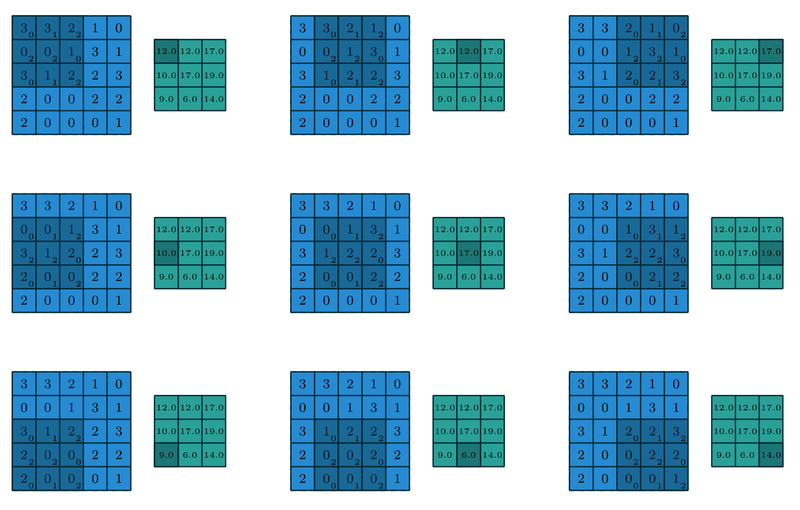
\includegraphics[scale=1.5]{assets/convolution_example}
	\caption{Пример конволюции цифрового изображения}
	\label{conv}
\end{figure}

Вычисление функций $f(x,\;y)$ и $h(x,\;y)$ из выражения \ref{svertka} путем выполнения обратных действий приводит к получению большой системы уравнений, решение которой является нетривиальной и трудоемкой задачей. Упростить ее решение может \textit{теорема о свертке}, согласно которой операция свертки в пространственной области эквивалентна поэлементному умножению в частотной области:

\begin{equation}
	f(x,\;y) \oplus h(x,\;y) \longleftrightarrow F(u,\;v) \cdot H(u,\;v),
\end{equation}

где $F(u,\;v)$, $H(u,\;v)$ --- Фурье~--~образы (спектры) функций $f(x,\;y)$ и $h(x,\;y)$ соответственно.

\clearpage

\section{Методы восстановления дефокусированных изображений}

Модель процесса получения дефокусированного цифрового изображения в пространственной области может быть представлена в виде выражения~(1.16)~\cite{equ}:

\begin{equation}
	g(x,\;y) = f(x,\;y) \oplus h(x,\;y) + \eta(x,\;y), 
\end{equation}

где:

\begin{enumerate}
	\item $f(x,\;y)$ --- функция, описывающая исходное (неискаженное) изображение.
	\item $g(x,\;y)$ --- функция, описывающая дефокусированное (искаженное) изображение.
	\item $h(x,\;y)$ --- функция размытия точки (в общем случае функция импульсного отклика).
	\item $\eta(x,\;y)$ --- функция шума.
	\item Символ <<$\oplus$>> --- оператор свертки. 
\end{enumerate}

Задача восстановления изображения заключается в поиске наилучшего приближения $\hat{f}(x,\;y)$ исходного изображения. Методы, решающие поставленную задачу, делятся на два класса в зависимости от наличия априорной информации о параметрах искажения.

\subsection{Методы классической деконволюции}

\subsubsection{Инверсный фильтр}

Одним из самых простых методов решения задачи деконволюции является инверсная фильтрация.

Согласно теореме о свертке, имеем (\ref{inv}):

\begin{equation}\label{inv}
	G(u,\;v) = F(u,\;v) \cdot H(u,\;v) + N(u,\;v).
\end{equation}

Было предложено разделить обе части выражения на $H(u,\;v)$ и получить следующую оценку исходного изображения:

\begin{equation}\label{inv_div}
	\hat{F}(u,\;v) = \cfrac{G(u,\;v)}{H(u,\;v)} = F(u,\;v) + \frac{N(u,\;v)}{H(u,\;v)}.
\end{equation}

Если на изображении отсутствует шум, то восстановление происходит достаточно точно. Однако, если шум присутствует, то составляющая $\cfrac{N(u,\;v)}{H(u,\;v)}$ стремится к бесконечности в виду того, что в частотной области $H(u,\;v)$ стремится к нулю, что приводит к получению некачественного результата~\cite{inv_noise}. Даже при малом шуме, который практически не заметен на изображении, результат содержит существенные помехи. 

Таким образом, данный метод практически никогда не применяется в реальных условиях.

\subsubsection{Фильтр Винера}

Усовершенствованием инверсной фильтрации можно считать фильтр Винера~\cite{winer}. Данный метод, в отличие от предыдущего, учитывает информацию о шуме на изображении.

Метод базируется на рассмотрении функций изображения и шума как случайных процессов и нахождении такой оценки $\hat{F}(u,\;v)$ для неискаженного изображения $f(x,\;y)$, чтобы среднеквадратическое отклонение этих величин было минимальным:

\begin{equation}
	\hat{F}(u,\;v) = \cfrac{1}{H(u,\;v)}\cdot\cfrac{|H(u,\;v)|^2}{|H(u,\;v)|^2+\cfrac{S_{\eta}(u,\;v)}{S_{f}(u,\;v)}}\cdot G(u,\;v).
\end{equation}

Функциями $S{\eta}$ и $S_f$ обозначают энергетические спектры шума и исходного изображения соответственно. Т.~к. эти величины обычно неизвестны, то их заменяют на некоторую константу $K$, которую можно охарактеризовать как приблизительное соотношение сигнал~--~шум:

\begin{equation}
	\hat{F}(u,\;v) = \frac{1}{H(u,\;v)}\cdot \frac{|H(u,\;v)|^2}{|H(u,\;v)|^2 + K} \cdot G(u,\;v).
\end{equation}

\clearpage 

На рисунках \ref{Fig:inv_1} и \ref{Fig:inv_2} представлен пример восстановления дефокусированного изображения с наличием шумовой составляющей.

\begin{figure}[!htb]
	\begin{minipage}{0.48\textwidth}
		\centering
		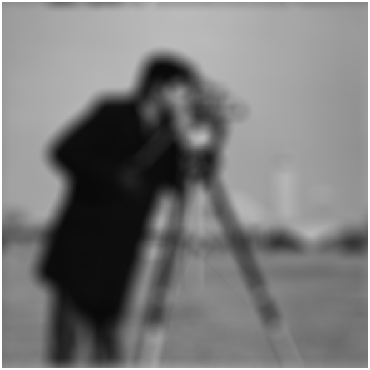
\includegraphics[scale=0.66]{assets/cameramen_wnr_before}
		\caption{Размытое и зашумленное изображение}\label{Fig:inv_1}
	\end{minipage}\hfill
	\begin{minipage}{0.48\textwidth}
		\centering
		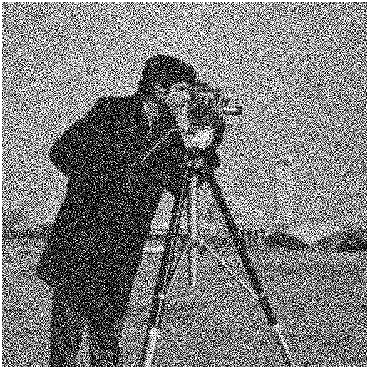
\includegraphics[scale=0.65]{assets/cameramen_wnr}
		\caption{Результат восстановления фильтром Винера}\label{Fig:inv_2}
	\end{minipage}
\end{figure}

Если шум на изображении отсутствует, то фильтр Винера сводится к инверсной фильтрации. Фильтр Винера эффективен для снижения шума и искажений, особенно когда статистические характеристики шума и искажений известны или могут быть оценены. Однако он предполагает линейность и стационарность сигнала и шума, что может быть ограничением в некоторых реальных ситуациях.

Важно отметить, что фильтр Винера может быть применен не только для восстановления изображений, но и для других типов сигналов, таких как аудио или временные ряды, где присутствуют шумы и искажения.

\subsubsection{Регуляризация по Тихонову}

Метод также реализовывается в частотной области. Этот метод также называют методом минимизации сглаживающего функционала со связью, или методом наименьших квадратов со связью.

Идея заключается в формулировке задачи в матричном виде с дальнейшим решением соответствующей задачи оптимизации. Решение задачи имеет следующий вид:

\begin{equation}
	\hat{F}(u,\;v) = \frac{H'(u,\;v)}{|H(u,\;v)|^2 + \gamma|P(u,\;v)|^2} \cdot G(u,\;v),
\end{equation}

где $\gamma$ --- параметр регуляризации, $P(u,\;v)$ --- результат Фурье~--~преобразования оператора Лапласа, $H'(u,\;v)$ --- функция, комплексно сопряженная $H(u,\;v)$.

На рисунках \ref{Fig:reg_1} и \ref{Fig:reg_2} представлен пример восстановления дефокусированного изображения с наличием шумовой составляющей.

\begin{figure}[!htb]
	\begin{minipage}{0.48\textwidth}
		\centering
		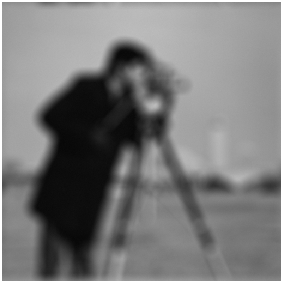
\includegraphics[scale=0.91]{assets/cameramen_reg_before}
		\caption{Искаженное изображение}\label{Fig:reg_1}
	\end{minipage}\hfill
	\begin{minipage}{0.48\textwidth}
		\centering
		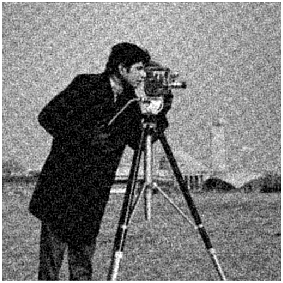
\includegraphics[scale=0.9]{assets/cameramen_reg}
		\caption{Результат восстановления}\label{Fig:reg_2}
	\end{minipage}
\end{figure}

Важным является вопрос выбора параметра регуляризации $\gamma$, сводящего поставленную задачу восстановления изображения к корректной. Если параметр $\gamma = 0$, то данный метод сводится к инверсной фильтрации.

Метод регуляризации Тихонова применяется для борьбы с проблемой неоднозначности восстановления и ограничениям, связанным с обратной задачей. Этот метод предполагает минимизацию суммы квадратов ошибок и квадратов регуляризационных членов в целевой функции.

Одним из преимуществ регуляризации Тихонова является возможность контролировать компромисс между точностью восстановления и сглаживанием. Параметр регуляризации, также называемый коэффициентом регуляризации, позволяет настраивать важность регуляризационного члена относительно суммы квадратов ошибок.

Если параметр регуляризации слишком большой, то сглаживание будет слишком сильным и могут быть потеряны важные детали. С другой стороны, если параметр регуляризации слишком мал, то артефакты могут сохраниться в восстановленном результате.

%Использование регуляризации Тихонова позволяет улучшить устойчивость и качество восстановления изображений в обратных задачах, особенно когда данные неоднозначны или зашумлены.

Все рассмотренные выше методы являются линейными и не итерационными, в следствие чего обладают одним общим недостатком --- чувствительностью к определению параметров искажения, т.е. в случае небольшого расхождения оценки искажающей функции качество восстановленного изображения резко ухудшается. Этому недостатку менее подвержен итерационный пространственный алгоритм Люси~--~Ричардсона.

\clearpage

\subsubsection{Метод Люси~---~Ричардсона}

Этот метод, в отличие от рассмотренных ранее, является итерационным, нелинейным и реализовывается в пространственной области.

Идея заключается в использовании метода максимального правдоподобия, для которого предполагается, что яркость изображения подчиняется распределению Пуассона. 

Математическое выражение для данного метода имеет следующий вид:

\begin{equation}
	\hat{f}_{k+1}(x,\;y) = \hat{f}_{k}(x,\;y) \cdot \left[h(-x,\;-y) \oplus \cfrac{g(x,\;y)}{h(x,\;y)\oplus \hat{f}(x,\;y)} \right], 
\end{equation}

где $\hat{f}_{k+1}(x,\;y)$ --- оценка изображения $f$ на $k$-ом шаге вычислений.

Т.к. обработка происходит в пространственной области, то нет необходимости в использовании преобразований Фурье, что позволяет снизить вычислительную сложность алгоритма.

На рисунках \ref{cam_blur} и \ref{cam_deblur} представлены искаженное (размытое и зашумленное) изображение и результат восстановления методом Люси~---~Ричардсона соответственно.

\begin{figure}[!htb]
	\begin{minipage}{0.48\textwidth}
		\centering
		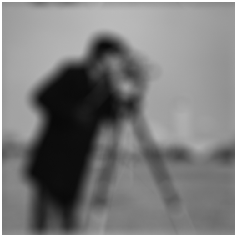
\includegraphics[scale=1.2]{assets/cameramen_blurred}
		\caption{Искаженное изображение}\label{cam_blur}
	\end{minipage}\hfill
	\begin{minipage}{0.48\textwidth}
		\centering
		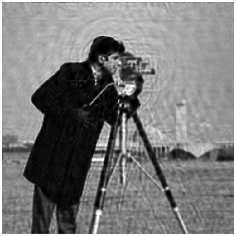
\includegraphics[scale=1.2]{assets/cameramen_deblurred}
		\caption{Результат восстановления}\label{cam_deblur}
	\end{minipage}
\end{figure}

Недостатком метода является возникновение краевых артефактов в виде горизонтальных и вертикальных полос на изображении. Также возникает вопрос об оптимальном количестве операций (выбор критерия остановки итерационного алгоритма).

\subsection{Сравнительный анализ методов классической деконволюции}

В рамках рассматриваемой задачи для метода классической деконволюции рассматриваются следующие критерии:

\begin{itemize}
	\item область вычислений --- пространственная или частотная;
	\item устойчивость к шуму на изображении;
	\item необходимость пост~-- или предобработки;
	\item сложность вычислений.
\end{itemize}

Обозначим данные критерии как $K1$, $K2$, $K3$ и $K4$ соответственно.

В таблице \ref{analys} представлен сравнительный анализ методов классической деконволюции.

\renewcommand{\arraystretch}{2}
\begin{table}[h!]
	\begin{center}
		\caption{Сравнительный анализ методов классической деконволюции}
		""\newline
		\label{analys}
		\begin{tabular}{ |c|c|c|c|c| } 
			\hline
			\textbf{Метод} & \textbf{$K1$} & \textbf{$K2$}& \textbf{$K3$}& \textbf{$K4$}\\
			\hline
			\textit{Инверсная фильтрация} & Частотная & Низкая & Нет & Низкая\\
			\hline
			\textit{Фильтр Винера} & Частотная & Низкая & Нет & Низкая\\
			\hline
			\textit{Метод Люси~--~Ричардсона} & Пространственная & Средняя & Да & Средняя\\
			\hline
			\textit{Регуляризация} & Частотная & Высокая & Да & Высокая\\
			\hline
		\end{tabular}
	\end{center}
\end{table}

Инверсный фильтр практически никогда не применяется в обработке реальных изображений, т.к. не учитывает наличие шума. Фильтр Винера является улучшением метода инферсной фильтрации, однако также устойчивость к шуму остается неудовлетворительной в реальных задачах, т.к. предполагает наличие информации о модели шума.

Метод Люси~--~Ричардсона является итерационным, в связи с чем имеет относительно высокую вычислительную сложность, однако является более устойчивым по отношению к шумовому компоненту.

Регуляризация Тихонова является наиболее стабильным методом, однако требует существенной нетривиальной предобработки изображения и имеет высокую вычислительную сложность.

\subsection{Подходы к решению задачи <<слепой>> деконволюции}

На практике информация об искажении практически никогда не бывает известна заранее, поэтому в данной работе будет разработан метод, учитывающий отсутствие любой априорной информации. Такая задача порождает целое семейство методов, которые называются методами <<слепой>> деконволюции. 

%Поставленная задача является некорректной --- количество неизвестных параметров превышает количество известных. 

В основе реализации методов <<слепой>> деконволюции лежат методы классической деконволюции, предполагающие наличие информации об искажении, базирующихся на методе максимального правдоподобия, где целевой функцией является исходное (неискаженное) изображение.

Как правило, метод состоит из трех этапов: 

\begin{enumerate}
	\item Ядро искажения оценивается по входному изображению.
	\item Используя оценочное ядро, применяется стандартный алгоритм деконволюции для оценки скрытого изображения.
	\item Оценка качества восстановленного сигнала.
\end{enumerate}

Методы слепой деконволюции могут использовать различные подходы, такие как статистическая оценка, регуляризация или использование априорной информации о свойствах исходного сигнала.

Существует два основных подхода к решению задачи вычисления <<слепой>> деконволюции~\cite{blind_def}:

\begin{enumerate}
	\item \textit{Определение ФРТ отдельно от восстанавливаемого изображения.} Полученная информация используется после применения одного из известных классических методов восстановления. Оценка функции импульсного отклика и восстановление изображения --- это отдельные процедуры для данного подхода. Алгоритмы, используемые для реализации данного метода, являются вычислительно простыми. 
	
	В таких случаях обычно матрица, соответствующая функции рассеяния точки, может быть иницализирована некоторыми стандартными значениями (часто выбирается значение $\cfrac{1}{N}$, где $N$ --- размерность квадратной матрицы ФРТ).  
	
	\item \textit{Включение идентификационной процедуры ФРТ в восстаналивающий алгоритм.} Этот подход подразумевает одновременную оценку функции импульсного отклика и восстанавливаемого изображения, что приводит к более сложным вычислительным алгоритмам.
\end{enumerate}

Целью задачи слепой деконволюции является получение функции исходного неискаженного изображения $f(x, \;y)$, и, соответственно, искажающей функции $h(x, \;y)$, которая была применена к изображению, зная только функцию искаженного изображения $g(x, \;y)$. 

\section{Методы оценки качества восстановления цифрового изображения}

Существует несколько методов оценки качества восстановленного дефокусированного изображения:

\begin{itemize}
	\item \textit{Пиковое отношение сигнал~--~шум} (англ. PSNR --- Peak Signal--to--Noise Ratio) --- скалярная метрика, обозначающая соотношение между максимальной мощностью сигнала и шума. Для вычисления PSNR чаще всего используется среднеквадратичная ошибка (англ. Mean Square Error). Метрика выражается в логарифмической шкале и измеряется в децибелах. Чем меньше значение этой метрики, тем хуже качество восстановления. 
	
	Является основным количественным критерием для оценки эффективности восстановления сигналов в виду, однако имеет ряд ограничений, основным из которых является тот факт, что PSNR (и MSE в частности) слабо коррелируют с физиологией человеческого восприятия.
	\item \textit{Индекс SSIM }(англ. Structure Similarity Index) характеризует структурное сходство между оригинальным и восстановленным сигналами, принимает значение в диапазоне от -1 до 1, где 1 соответствует совпадению оригинального сигнала с восстановленным, а -1 --- полному различию сигналов. Метрика учитывает яркость, контрастность и структуру изображения.
	\item\textit{ Метрика оценки восприятия человека} (англ. HPM --- Human Perception Metric) характеризует качество восстановленного сигнала на основе психофизиологических особенностей восприятия сигналов человеком. Является наиболее трудозатратной, т.к. требует участие людей в проведении эксперимента и анализе данных, однако является наиболее достоверной.
\end{itemize}

%1. Метрика оценки остроты изображения (Image Sharpness Metric): Эта метрика использует статистические методы для оценки остроты изображения, чтобы измерить качество восстановления дефокусированного изображения. Метрика оценки остроты изображения часто используется для оценки качества восстановления дефокусированных изображений.
%
%2. Метрика оценки контрастности изображения (Image Contrast Metric): Эта метрика оценивает контрастность изображения, чтобы измерить качество восстановления дефокусированного изображения. Метрика оценки контрастности изображения также часто используется для оценки качества восстановления дефокусированных изображений.
%

Выбор метрики оценки качества восстановления дефокусированного изображения зависит от конкретной задачи и требований к качеству восстановленного изображения.

\section{Постановка задачи}

На рисунке \ref{fig:idef0} представлена IDEF0 диаграмма уровня A0 для метода восстановления дефокусированных изображений на основе определенных параметров искажения. 

\begin{figure}[H]
	\centering
	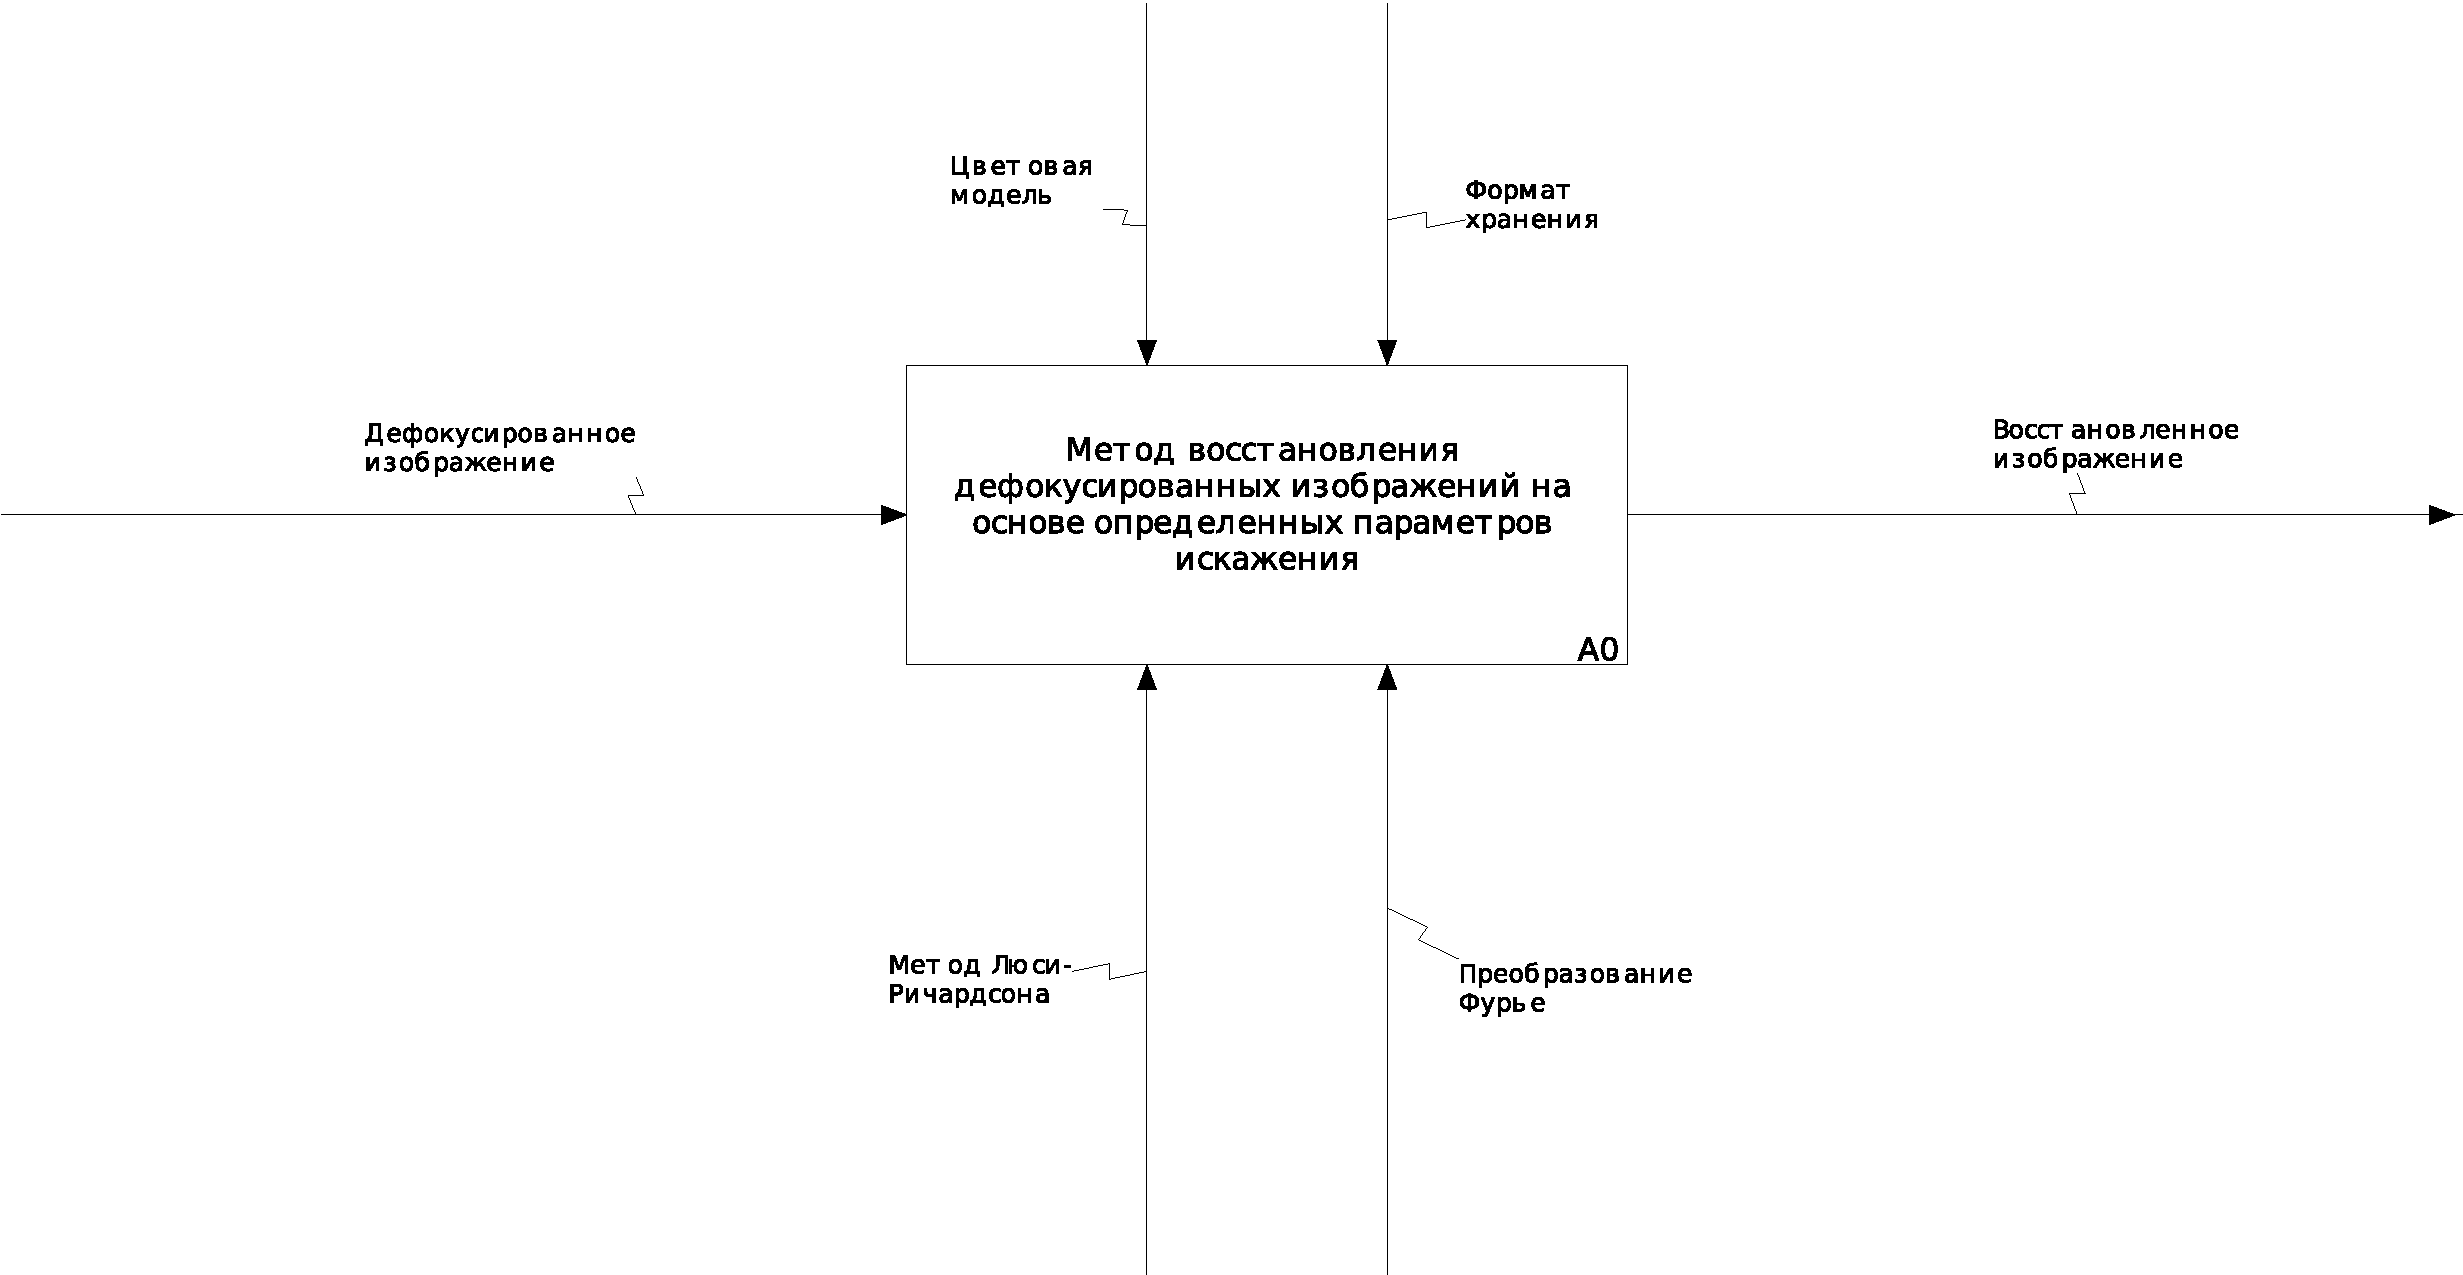
\includegraphics[scale=0.4]{assets/01_A0}
	\caption{IDEF0 диаграмма уровня А0}
	\label{fig:idef0}
\end{figure}

\section*{Выводы}

В данном разделе были рассмотрены основные понятия предметной области, а также методы деконволюции с учетом априорной информации об искажении, а также при ее отсутствии.

В качестве цветовой модели цифрового изображения была выбрана модель RGB, т.к. разрабатываемый метод является линейным, т.е. при обработке непосредственно самого изображения нет необходимости обрабатывать какие~-~либо локальные подобласти.

В качестве форматов хранения выбраны расширения PNG, JPG и BMP как наиболее распространенные форматы хранения цифровых изображений, получаемых при съемке фотокамерой.

Для оценки качества восстановления будут использованы метрики PSNR (пиковое отношение сигнал~--~шум) и HPM (оценка восприятия человека). В рамках рассматриваемой задачи метрика SSIM является неприменимой, т.к. по условию отсутствует априорная информация об искажении, а в частности и оригинальное изображение~\cite{psnr_ssim}. 

Метрика PSNR позволяет автоматизировать процесс оченки качества восстановления, однако эта оценка неполная, т.к. не учитывает особенности психофизиологического восприятия человеком сигнала. Наиболее точной в рамках поставленной задачи будет метрика HPM. В рамках поставленной задачи в роли эксперта выступает автор работы.

В качестве метода классической деконволюции был выбран метод Люси~--~Ричардсона, т.к. фильтр Винера существенно чувствителен к шуму и статистической информации о нем, а метод регуляризации Тихонова имеет высокую вычислительную сложность и требует предварительную нетривиальную оценку параметров регуляризации для изображения. Выбранный метод является применимым, когда модель искажения может быть оценена, в частности в случае дефокусировки эта оценка возможна.

Процесс слепой деконволюции обычно включает в себя оценку неизвестной функции свертки и восстановление исходного сигнала. В качестве подхода к решению задачи <<слепой>> деконволюции было решено определять ФРТ на основе кепстрального анализа, который в свою очередь базируется на анализе амплитудной составляющей спектра исходного изображения. 

Было выяснено, что функция рассеяния точки в случае дефокусировки фотокамеры имеет форму диска, радиус которого равен радиусу дефокусировки, а структура кепстра содержит кольца, радиус которых зависит от степени дефокусировки.

Важно отметить, что слепая деконволюция является сложной задачей, особенно при наличии шума или других искажений в наблюдаемых данных, а также имеет ряд особенностей и ограничений, в связи с чем в дальнейшем необходимо определить область применимости предлагаемого метода восстановления.